\section{Evaluation} \label{sec:evaluation}
%todo put method in here, if it stays small

\subsection{Memory-based Unbalanced tree search}
%Traversal of an unbalanced, unpartitioned tree captures the foundations for implementing most forms of irregular parallelism. 
...
%Recursion is found in every irregular divide and conquer algorithm. Loops, even regular ones, must be dynamically scheduled to get good load balance when run on a large, non-uniform system. Nested parallelism involves fine-grain creation of dynamic amounts of work. Dataflow..

Unbalanced tree search (UTS), is a benchmark for evaluating the programmability and performance of systems for parallel applications that require dynamic load balancing \cite{Olivier:uts2006}. It involves traversing an unbalanced implicit tree: at each vertex, its number of children is sampled from some probability distribution, and this number of new nodes are added to a work queue to be visited. While this benchmark captures irregular, dynamic parallelism, we want to evaluate performance on algorithms that touch existing data. We augment UTS by using the traversal to create a large tree in memory, and then we traverse the in-memory tree. We call this benchmark UTS-mem, and the timed portion is this traversal of the in-memory tree. The assumption is that in general the size of each subtree is unknown until that subtree has actually been traversed.

%todo: say tree explore is same as a search except we are additionally needing to synchronize on all vertices visited

The Grappa version of tree search UTS-mem

\lstset{language=C++,
       basicstyle=\footnotesize,
       tabsize=2}
\begin{lstlisting}
// base of shared vertex_t[]
GlobalAddress<vertex_t> Vertices;        

// base of shared int64_t[]
GlobalAddress<int64_t> ChildrenPointers;  

void search_vertex( id ) {
  GlobalAddress<vertex_t> v_addr = Vertices + id;
  Incoherent<vertex_t>::RO v( v_add, 1 );

  // start index of my children pointers
  childIndex = v->childIndex;    

  // how many children I have
  numChildren = v->numChildren;  

  // parallel loop over the child list for this vertex
  parallel_for(fn=&search_children, start=childIndex, iters=numChildren);
}

void search_children( start, iters ) {
  // take advantage of spatial locality in the array of children
  GlobalAddress<int64_t> child_base_addr = ChildrenPointers + start;
  Incoherent<int64_t>::RO childIds( child_base_addr, iters );

  // spawn a task to visit each child
  for (i = 0..iters) {
    SoftXMT_publicTask( fn=&search_vertex, id=childIds[i] );
  }
}
\end{lstlisting}

We ran UTS-mem on Grappa and the XMT with two different 100M-vertex trees with a geometric distribution numChildren distribution. Figure~\ref{fig:grappa-xmt-uts} shows the performance in terms of number of vertices visited per second versus number of compute nodes. The Grappa results are for the best parameter values from a limited search over \flushtimeout~and \asyncforthr~\TODO{want to say this in general at beginning of eval?}. Grappa achieves 3x better performance for 12 nodes. Scaling up, Grappa adds 2Mvert/s/node versus XMT's 850Kvert/s/node.
\TODO{why is XMT getting different results for T1L,T2L; would expect it to be the machine with the most uniform results.}

\TODO{sensitivity study for \asyncforthr parameter, ie caching amount. Although we can take advantage of locality in children array and the XMT cannot, we still win without it}


\begin{figure}[h]
    \begin{center}
        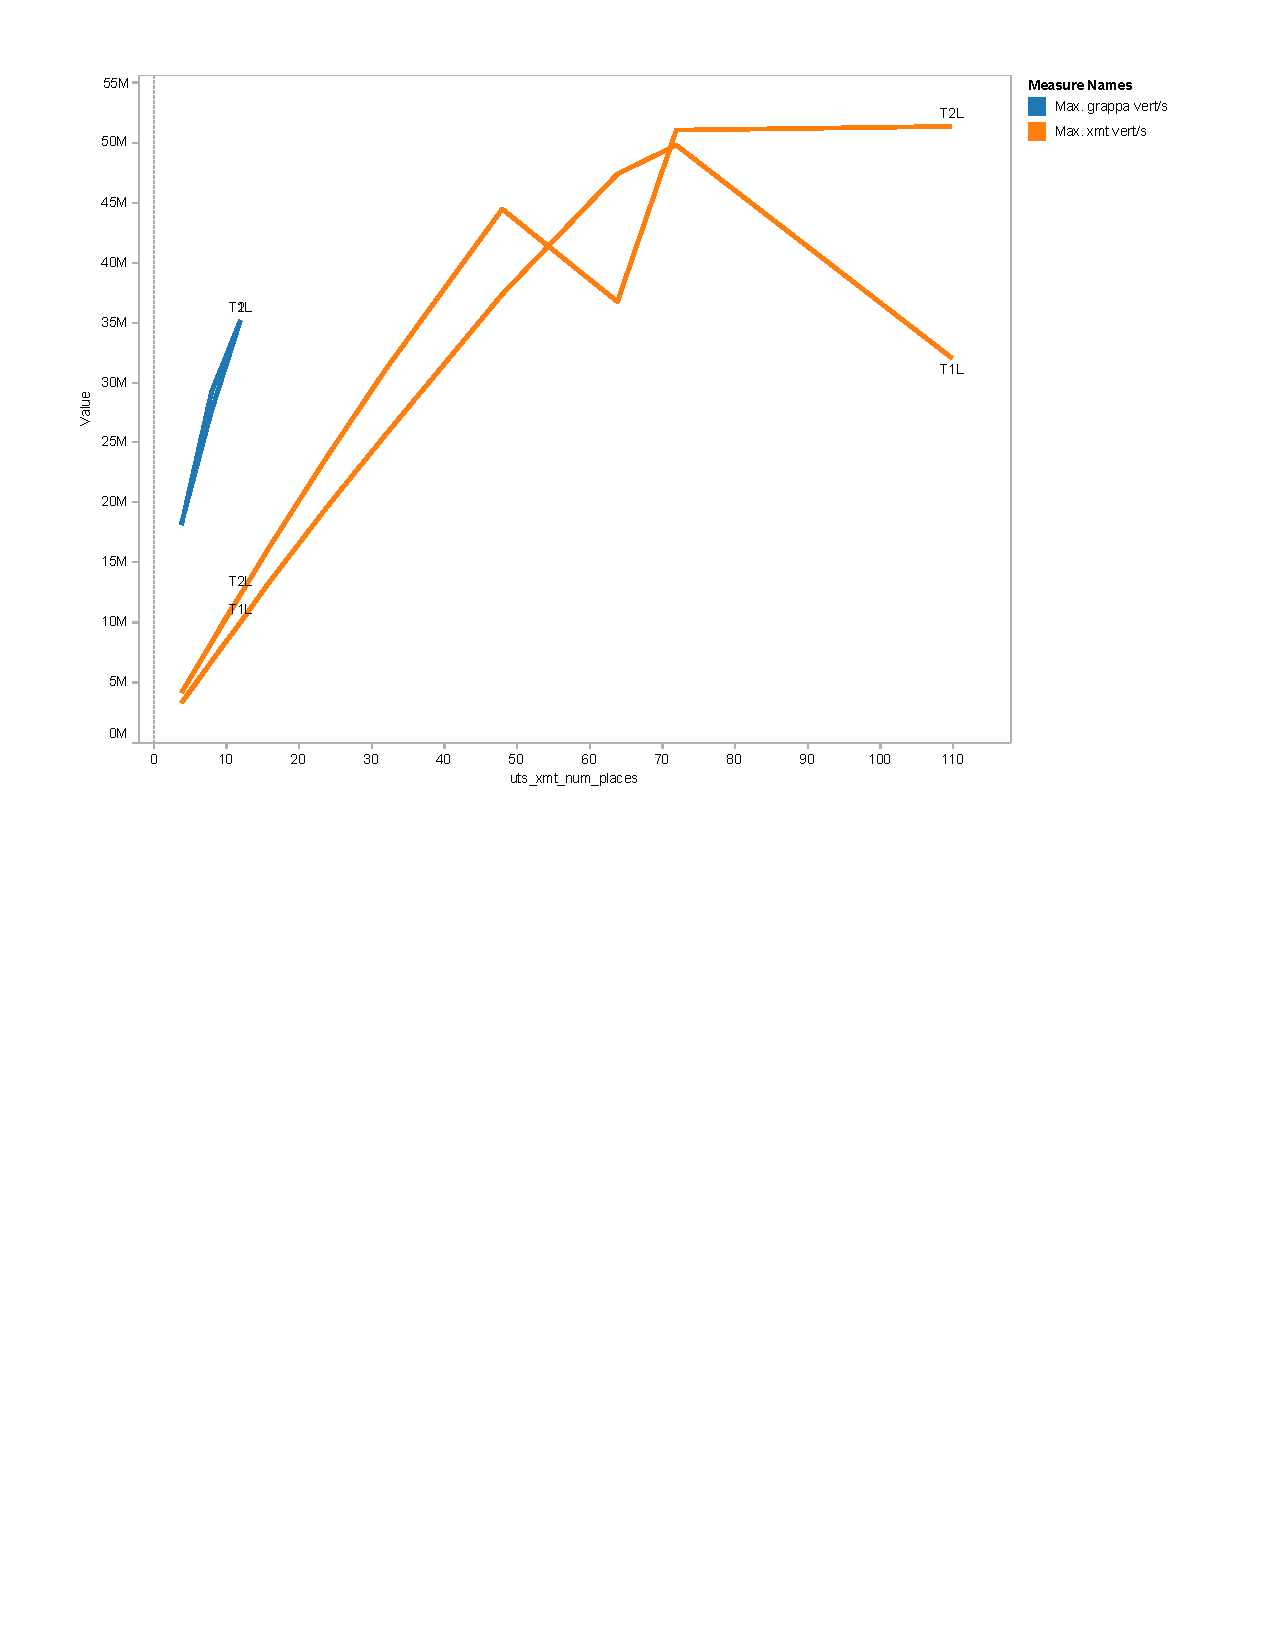
\includegraphics[width=0.5\textwidth]{figs/grappa-xmt-uts.pdf}
    \end{center}
    \caption{describe...}
    \label{fig:grappa-xmt-uts}
\end{figure}


